\chapter{Summary \& Reflections}


% Including a discussion of results in a wider context (considering other work).


\section{Project management}

% Covering the tasks as a part of your work plan and progress as well as how time and resources are managed.
As outlined in the project plan, the project is being managed using the Kanban Agile methodology \cite{stellman2014learning}. Kanban has allowed for the flexibility of being able to take any card from the project backlog at any time, which has been ideal for this project as the research undertaken, and the lessons learnt from building prototypes has dictated changes to the direction of the work at various times. 

An online Kanban board has been set up on Trello, with `Backlog', `On Hold', `In Progress', and `Done' columns. When new tasks are identified, they are added to the `Backlog' column. The `On Hold' column is for tasks that were previously `In Progress', but for which work cannot continue until some other, previously unidentified, task is completed. When the blocking task is complete, the `On Hold' task is returned to `In Progress'.

\begin{figure}[h!]
  \centering
  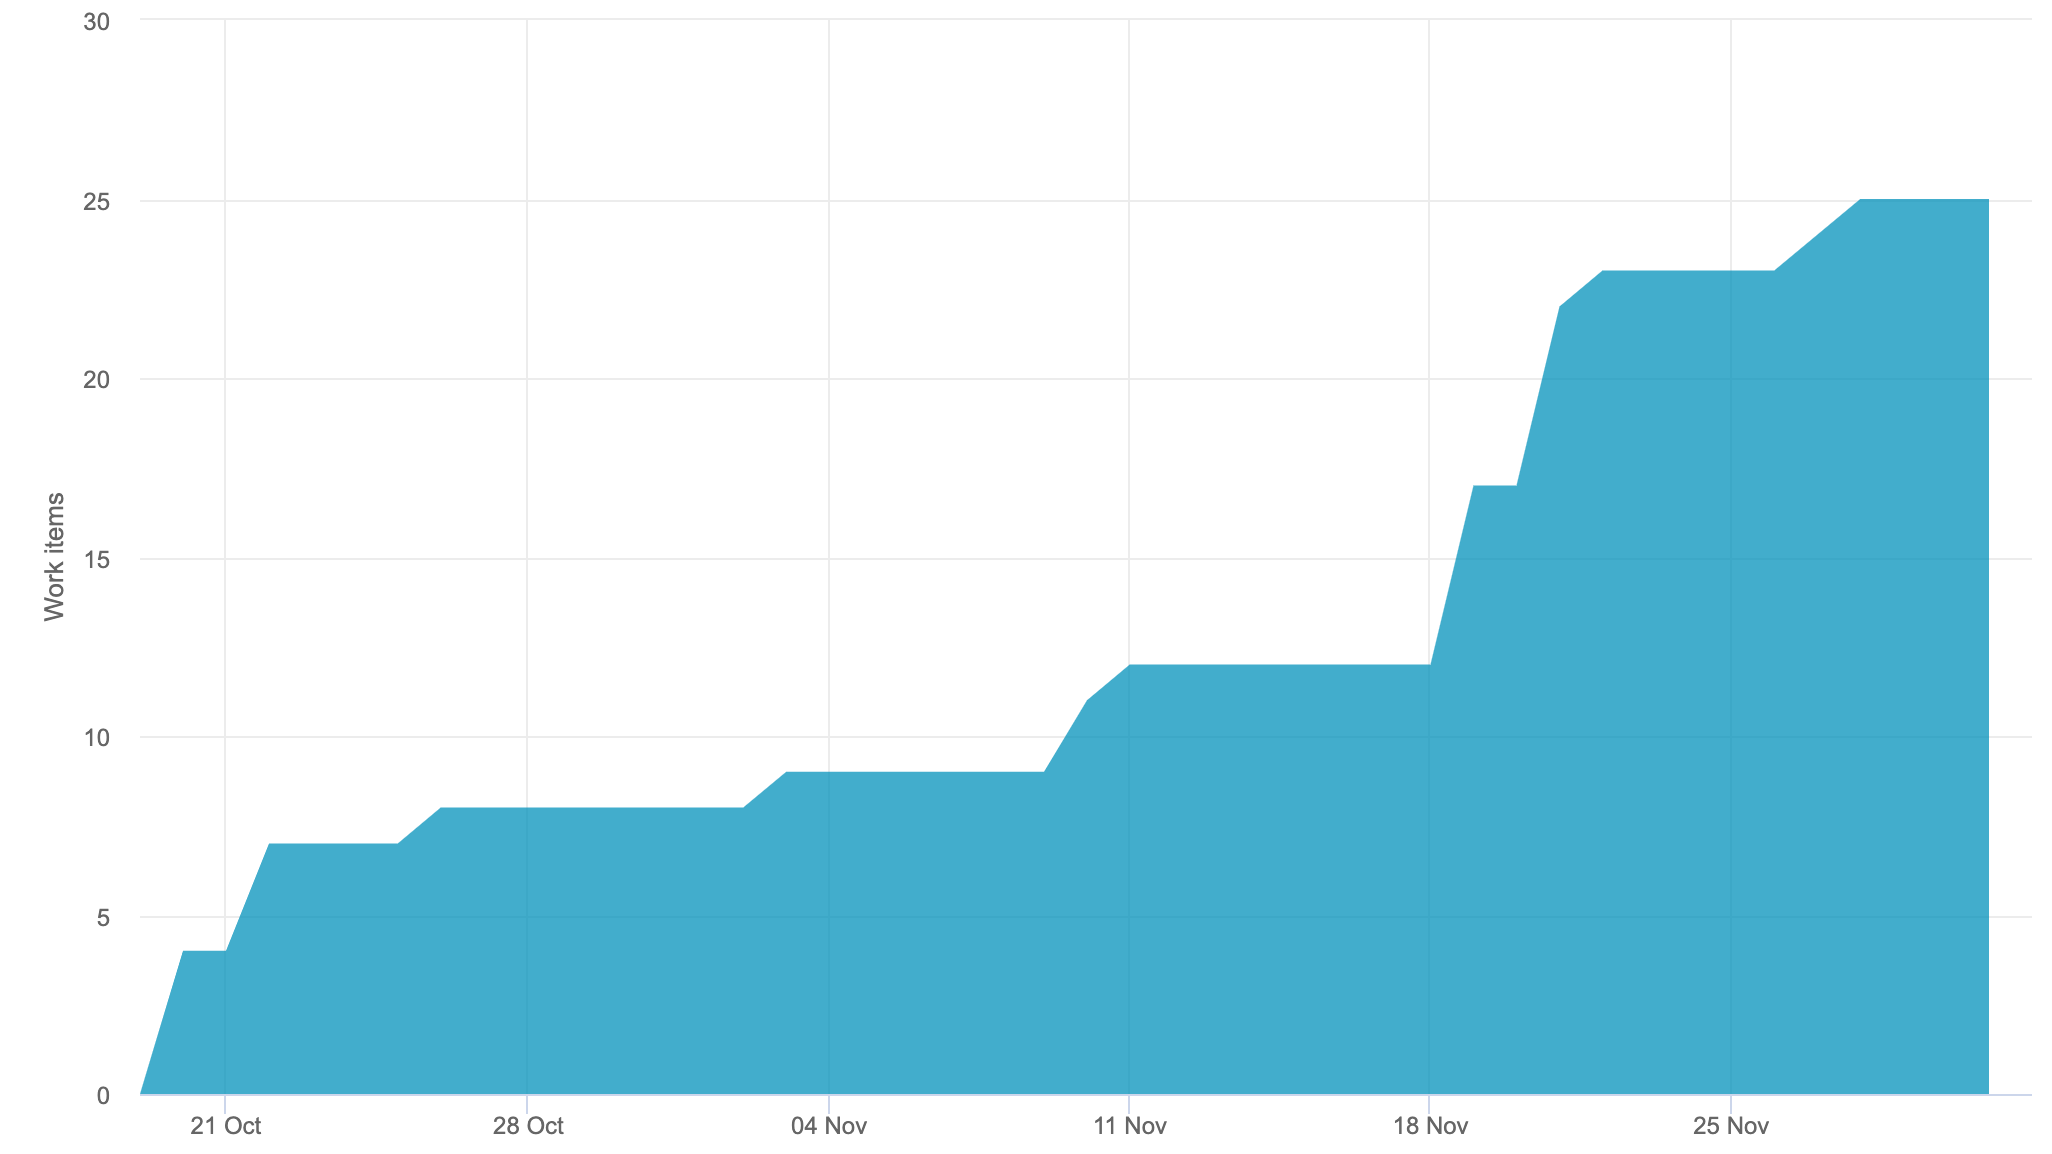
\includegraphics[width=\textwidth]{images/burnup.png}
  \caption{Graph showing number of completed work items over time}
  \label{fig:burnup}
\end{figure}

Work over the course of the project so far has been consistent, with task completion being spread out over time, as illustrated in Figure \ref{fig:burnup}. The mean Cycle Time, i.e. the amount of time that a task spends either `In Progress' or `On Hold' \cite{roock2010kanban}, is currently 4.2 days, with 85\% of tasks having a cycle time of 8 days or fewer.

Due to the fact that the project is currently on schedule, with no perceived setbacks in the near future, it is not deemed necessary to make any adjustments to the work plan at this time. Progress will be reviewed regularly so that changes to the schedule can be made if and when necessary.

\section{Contributions and reflections}

% Providing the details of your achievements and contributions including innovation, creativity and novelty (if there is any) as well as a personal reflection on the plan and your experience of the project (a critical appraisal of how the project went).
The creation of a user interface, alongside the prototype for sending and receiving emails mean that significant progress has been made towards achieving the objectives of the project. It should be noted that the second semester contains fewer credits from other modules than the first, and therefore more time will be allocated per week to this project in the second semester. This is a factor that was considered when estimating time for tasks in the project plan. The project is progressing at a good pace, on track with the initial proposed timeline. This suggests that the amount of time-effort for each task has been estimated accurately, and therefore it is believed that the full scope of the project can be completed within the time constraints.

I believe that the implementation work that has been completed so far is of a high quality, however there is room for improvement in the quality of documentation, and this will be a focus moving forward.

\section{Future Work}
